\subsection{Response-only quality comparison}
Each value is mean teacher-forced response loss in nats per scored token over
64 paired examples. The two response candidates start from the same parent
weights and receive the same 32 response-masked batches; the larger candidate
first adds four identity-initialized blocks.
\begin{center}\small
\begin{tabular}{lrrr}\toprule
Checkpoint & Retention & Fresh & Untouched test\\\midrule
Original seed (135M) & 1.325133 & 1.281919 & 1.285737\\
Prefix-trained parent (135M) & 1.325136 & 1.284188 & 1.285587\\
Response-trained candidate (135M) & 1.324262 & 1.282754 & 1.285286\\
Response-trained candidate (149M) & 1.324338 & 1.282783 & 1.285116\\
\bottomrule\end{tabular}\end{center}
Neither response candidate passes the predefined promotion gate. Relative to
their common parent, fresh-loss changes are -0.001434 and -0.001405 nats, but
their approximate 99\% upper bounds are +0.000639 and +0.000596; the required
bound is below -0.001. The larger candidate has no demonstrated fresh-loss
advantage over the smaller candidate under the same training budget. Relative
to the original seed, both candidates also fail the improvement gate.
These are negative promotion results, not evidence of continual capability
improvement. All candidates produced the same tested 32-token greedy answer
prefix to the single solar-panel prompt; that anecdotal output is not a quality
benchmark. The chosen thresholds were not relaxed after observing these results.
\begin{figure}[ht]\centering
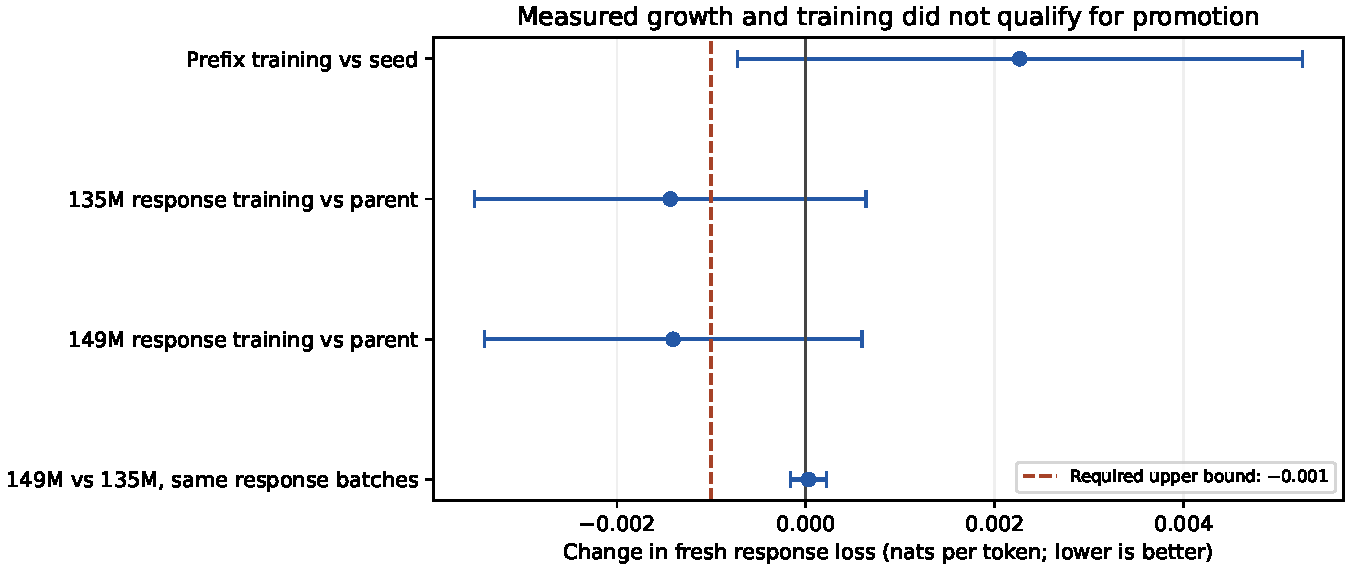
\includegraphics[width=.97\linewidth]{eval/results/evolution20260911/response-quality.pdf}
\caption{Paired fresh-response loss changes with approximate 99\% normal
intervals, 64 examples per comparison. Lower is better. Every interval crosses
zero; none establishes the required improvement. Intervals are not corrected
for multiple comparisons.}\end{figure}
